\chapter{Supplementary materials}
\section{Description of the computational cluster used in the work}
\label{cluster}


\section{Supplementary materials for \autoref{chap:CMZ}}
\subsection{Developmental progression of naso-temporal population asymmetry in the CMZ}

\begin{figure}[!h]
    \makebox[\textwidth][c]{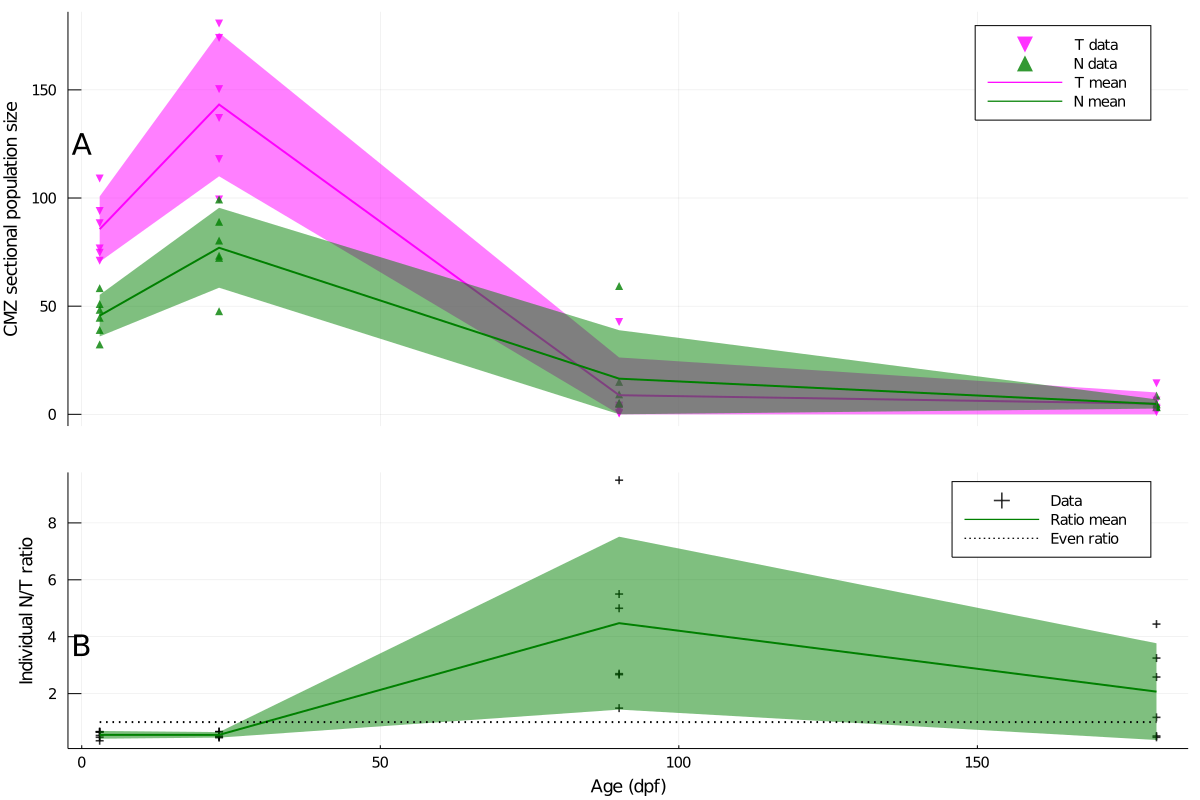
\includegraphics[width=1.2\textwidth]{cmz/NTontology.png}}    
    \caption{{\bf Developmental progression of naso-temporal population asymmetry in the CMZ.}}
    Marginal posterior distribution of mean nasal (N) and temporal (T) population size in 14$\mu$m transverse cryosections (panel A) or intra-individual N/T count asymmetry ratio (panel B), $\pm 95\%$ credible interval, n=6 animals per age. Data points represent mean counts from three central sections of an experimental animal's eye. 
    \label{NTontology}
\end{figure}


\subsection{Methods}
\label{ssec:CMZmethods}

\subsubsection{Statistical Analyses}
We calculate the 



% \section{Supplementary materials for \autoref{chap:rys}}
% \subsection{A frequentist clustering analysis of the rys nucleosome position data produces meaningful-looking but useless data}

% % \subsection{Notes on using BioBackgroundModels}

% \subsection{Notes on using BioMotifInference}

% Skilling's nested sampling algorithm is mathematically guaranteed to converge an ensemble of models on the global optimum likelihood in the parameter space\cite{Skilling2006}. Skilling acknowledges at least one assumption underpinning this guarantee, which is that the sampling density (in effect, the size of the ensemble) be high enough that widely separated modes are populated by at least one model each. Although early suggestions for the generation of new models within the ensemble were generally to decorrelate existing models by \hyperref[MonteCarlo]{Monte Carlo} permutation, later work generally acknowledges that this can be highly inefficient, particularly in large parameter spaces with many modes, of which the sequence parameter spaces explored in \autoref{chap:rys} are good examples. A number of ways of addressing this problem have arisen in the cosmology and physics literature. These include methods of improving model generation, such as sampling within an ellipsoidal hypersphere encompassing the positions of the ensemble models within the parameter space \cite{Feroz2008,Feroz2009} or Galiliean Monte Carlo (GMC) \cite{Skilling2012}, as well as methods of increasing computational efficiency, such as dyamic adjustment of ensemble size \cite{Higson2019}. 

% Generally speaking, these methods are not available to us because the PWM representation of sequence signal in the ICA PWM model (IPM) is not readily susceptible to parameter space analysis. This is for at least three reasons:

% \begin{enumerate}
%     \item Identical IPMs may be expressed with their vector of sources in different orders. Relating IPMs in parameter space is therefore difficult; it is unclear how one would define a hypersphere across the ensemble's parameters.
%     \item IPM sources may be of different lengths. Even if we can relate sources in different models to one another by some consistent distance rule, it is unclear how one would project shorter sources into the parameter space of longer ones, particularly given the first problem. BioMotifInference does maintain an index for each source against its prior, but this is no guarantee that sources remain in some way "aligned". Rather, some type of alignment would have to be done, probably massively increasing computational cost to questionable benefit.
%     \item If model likelihoods are being calculated on the reverse strand of observations, sources on opposite ends of the parameter space (ie. reverse complements) can represent closely equivalent signals.
% \end{enumerate}

% These issues make it difficult to see how one would mathematically describe the position of existing ensemble models within the parameter space at all, precluding sampling from a hypersphere or the use of GMC. Therefore, BioMotifInference (BMI), like it's predecessor nMICA, samples new models by applying one of a collection of permutation functions to an existing model. Additionally, although BMI is supplied prior distributions on ICA parameters from which the initial ensemble is sampled, there is no way to calculate a sensical posterior from the models generated by the nested sampling process. The primary outputs of interest are the estimation of the Bayesian evidence for model structure given the data, given as its logarithm, as well as the models in the final ensemble (which constitute samples around the posterior mode or modes).

% Because the more conventional methods to address the ineffiency of nested sampling by Monte Carlo used in cosmological models described above are unavailble, BMI uses an ad hoc method of adjusting the mixture of permute patterns that are applied to models. The basic permute logic (encoded by Permute_Instruct arguments to the permute_IPM function) is as follows:

% \begin{enumerate}
%     \item[selectmodel] Select a random  model from the ensemble.
%     \item[applyfunc] Apply a randomly selected permutation function from the instruction's function list according to the probability weights given to the functions by the instruction's weight vector.
%     \item Repeat \ref{applyfunc} until a model more likely than the ensemble contour, given observations, is found, or the instruction's func_limit is reached.
%     \item If the func_limit is reached without a new model being found, return to \ref{selectmodel} and repeat \ref{applyfunc} until a model more likely than the ensemble's contour is found, or until the instruction's model_limit is reached.
% \end{enumerate}